% !TEX program = xelatex
% 编译：在 docs/ 目录下执行   xelatex derivation.tex   （建议运行两遍以生成目录/交叉引用）
\documentclass[12pt]{ctexart}

\usepackage{amsmath,amssymb,amsthm,mathtools}
\usepackage{bm}
\usepackage{graphicx}
\usepackage{booktabs}
\usepackage{float}
\usepackage[a4paper,margin=2.4cm]{geometry}
\usepackage{enumitem}
\usepackage[hidelinks]{hyperref}

% ---- 记号约定 -----------------------------------------------------------
\newcommand{\R}{\mathbb{R}}
\newcommand{\w}{\bm{w}}
\newcommand{\muv}{\bm{\mu}}
\newcommand{\Sig}{\bm{\Sigma}}
\newcommand{\one}{\mathbf{1}}
\newcommand{\T}{^{\mathsf{T}}}
\newcommand{\Sinv}{\Sig^{-1}}
\DeclareMathOperator*{\argmin}{arg\,min}
\DeclareMathOperator{\tr}{tr}

\theoremstyle{definition}
\newtheorem{definition}{定义}
\theoremstyle{plain}
\newtheorem{theorem}{定理}
\newtheorem{proposition}{命题}
\newtheorem{lemma}{引理}

\title{\textbf{均值--方差投资组合的多目标规划：\\矩阵算法、解析解与投影梯度下降}}
\author{矩阵算法课程项目}
\date{\today}

\begin{document}
\maketitle

\begin{abstract}
本项目把量化金融中最经典的资产配置问题——Markowitz 均值--方差模型——建模为一个
\textbf{双目标规划问题}（同时最大化期望收益、最小化风险），并从\textbf{矩阵算法}的视角
给出完整推导与实现。我们：(1) 用拉格朗日乘子法与 KKT 条件导出允许卖空时有效前沿的
\textbf{闭式解}，核心是对对称正定协方差矩阵 $\Sig$ 的求逆/求解（Cholesky 分解）；
(2) 在加入不可卖空约束 $\w\ge\bm 0$ 后问题失去闭式解，于是\textbf{从零实现投影梯度下降}
（含单纯形欧氏投影的 KKT 推导与收敛性分析）；(3) 用 Ledoit--Wolf 收缩估计这一
\textbf{统计学习（机器学习）}方法改善 $\Sig$ 的估计，并定量展示其在小样本/高维时的价值。
全部结论在合成但统计特征真实的 8 资产数据上验证，并附 5 张图像。
\end{abstract}

\tableofcontents

% =========================================================================
\section{问题背景与现实意义}

设某投资者面对 $n$ 只股票，需决定把资金按比例 $\w=(w_1,\dots,w_n)\T$ 配置到各资产上
（$w_i$ 为第 $i$ 只股票的权重，$\sum_i w_i=1$）。投资者的两个目标天然冲突：

\begin{itemize}[nosep]
  \item \textbf{收益越高越好}：组合期望收益为 $\muv\T\w$，其中 $\muv\in\R^n$ 是各资产期望收益；
  \item \textbf{风险越低越好}：组合方差为 $\w\T\Sig\w$，其中 $\Sig\in\R^{n\times n}$ 是收益的协方差矩阵。
\end{itemize}

高收益资产往往伴随高波动，因此不存在同时让两者最优的单一解，而是一族\textbf{折中（Pareto）解}。
寻找这族解、并理解“多承担一单位风险能换来多少额外收益”，正是资产配置的核心，
也是一个标准的\textbf{多目标规划}问题。其数学骨架完全由矩阵运算构成（二次型、矩阵求逆、
特征分解），因此非常适合作为矩阵算法课程的综合案例。

% =========================================================================
\section{多目标规划建模}

\subsection{符号与假设}
记全 $1$ 向量为 $\one\in\R^n$。假设 $\Sig$ \textbf{对称正定}（$\Sig\succ 0$）——
这在样本协方差中当观测期数 $T>n$ 且无完全共线资产时几乎必然成立，也保证了二次型
$\w\T\Sig\w>0$（任意非零组合都有正风险）以及目标函数的\textbf{严格凸性}。

\subsection{双目标模型}
\begin{equation}
\min_{\w}\ \Big(\, \w\T\Sig\w,\ \ -\,\muv\T\w \,\Big)
\quad\text{s.t.}\quad \one\T\w=1,\quad (\text{可选})\ \w\ge\bm 0 .
\label{eq:biobj}
\end{equation}
约束 $\one\T\w=1$ 表示资金全部投出；$\w\ge\bm 0$ 表示\textbf{不可卖空}（只能买入）。

\begin{definition}[Pareto 最优]
可行解 $\w^\star$ 称为 Pareto 最优，若不存在另一可行解 $\w$ 使得两个目标都不更差、
且至少一个严格更优。所有 Pareto 最优组合在 $(\sigma,\,r)=(\sqrt{\w\T\Sig\w},\,\muv\T\w)$
平面上的像称为\textbf{有效前沿（efficient frontier）}。
\end{definition}

\subsection{标量化：把多目标化为单目标}
求解多目标规划的常用手段是\textbf{标量化}，即用一个标量参数把两目标合成一个目标，
扫描该参数即可得到整条前沿。本文用两种等价方式：

\paragraph{(a) 加权和法。}引入风险偏好系数 $\lambda\ge0$：
\begin{equation}
\min_{\w}\ \tfrac12\,\w\T\Sig\w-\lambda\,\muv\T\w \quad\text{s.t.}\quad \one\T\w=1 .
\label{eq:weighted}
\end{equation}
$\lambda=0$ 对应纯最小方差；$\lambda\to\infty$ 对应纯最大收益。

\paragraph{(b) $\varepsilon$--约束法。}固定一个目标收益 $r$，最小化风险：
\begin{equation}
\min_{\w}\ \tfrac12\,\w\T\Sig\w \quad\text{s.t.}\quad \muv\T\w=r,\ \ \one\T\w=1 .
\label{eq:eps}
\end{equation}
扫描 $r$ 即得前沿。由于 $\Sig\succ0$ 使目标严格凸、约束为线性，两种标量化都给出
\emph{唯一}全局最优，且其解集相同（KKT 充要）。下一节用 \eqref{eq:eps} 推导闭式解。

% =========================================================================
\section{解析解：拉格朗日乘子与 KKT 条件}
\label{sec:analytic}

\subsection{一阶最优性条件}
对 \eqref{eq:eps} 写拉格朗日函数（$\lambda,\gamma$ 为乘子）：
\begin{equation}
\mathcal L(\w,\lambda,\gamma)=\tfrac12\,\w\T\Sig\w-\lambda(\muv\T\w-r)-\gamma(\one\T\w-1).
\end{equation}
对 $\w$ 求梯度并令其为零（这就是等式约束下的 KKT 平稳性条件）：
\begin{equation}
\nabla_{\w}\mathcal L=\Sig\w-\lambda\muv-\gamma\one=\bm 0
\ \Longrightarrow\
\boxed{\ \w=\Sinv(\lambda\muv+\gamma\one)\ } .
\label{eq:wstar}
\end{equation}
因目标严格凸、约束线性，该平稳点即\textbf{全局最优}。

\subsection{消去乘子：一个 $2\times2$ 线性系统}
把 \eqref{eq:wstar} 代入两个约束，并定义四个由矩阵 $\Sig$ 决定的标量
\begin{equation}
A=\one\T\Sinv\muv,\qquad B=\muv\T\Sinv\muv,\qquad C=\one\T\Sinv\one,\qquad D=BC-A^2,
\label{eq:ABCD}
\end{equation}
得到
\begin{equation}
\begin{cases}
\muv\T\w=\lambda B+\gamma A=r,\\[2pt]
\one\T\w=\lambda A+\gamma C=1,
\end{cases}
\quad\Longleftrightarrow\quad
\begin{bmatrix}B & A\\ A & C\end{bmatrix}
\begin{bmatrix}\lambda\\ \gamma\end{bmatrix}
=\begin{bmatrix}r\\ 1\end{bmatrix}.
\end{equation}
该系数矩阵的行列式恰为 $D=BC-A^2$。由 Cauchy--Schwarz 不等式（在内积
$\langle\bm x,\bm y\rangle=\bm x\T\Sinv\bm y$ 下）可证 $D>0$（当 $\muv$ 与 $\one$ 线性无关），
故系统可解：
\begin{equation}
\lambda=\frac{Cr-A}{D},\qquad \gamma=\frac{B-Ar}{D}.
\label{eq:lamgam}
\end{equation}

\subsection{有效前沿的闭式表达}
最优组合的方差可由 \eqref{eq:wstar} 巧妙化简（利用 $\w\T\Sig\w=\w\T(\lambda\muv+\gamma\one)
=\lambda r+\gamma$）：
\begin{equation}
\boxed{\ \sigma^2(r)=\w\T\Sig\w=\frac{C\,r^2-2A\,r+B}{D}\ }.
\label{eq:frontier}
\end{equation}
这是 $(\sigma^2,r)$ 平面上的\textbf{抛物线}、$(\sigma,r)$ 平面上的\textbf{双曲线}——
即图\ref{fig:frontier} 中的有效前沿。其顶点（最小方差点）由 $\mathrm d\sigma^2/\mathrm dr=0$ 给出。

\subsection{两个关键组合}

\begin{proposition}[全局最小方差组合 GMV]
在 \eqref{eq:eps} 中去掉收益约束，只留 $\one\T\w=1$，解得
\begin{equation}
\w_{\mathrm{gmv}}=\frac{\Sinv\one}{\one\T\Sinv\one}=\frac{\Sinv\one}{C},\qquad
\sigma^2_{\mathrm{gmv}}=\frac1C,\qquad r_{\mathrm{gmv}}=\frac{A}{C}.
\end{equation}
\end{proposition}
\begin{proof}
由 $\Sig\w=\gamma\one$ 得 $\w=\gamma\Sinv\one$；代入 $\one\T\w=1$ 得 $\gamma=1/C$。
方差 $\w\T\Sig\w=\gamma^2\,\one\T\Sinv\one=C/C^2=1/C$。
\end{proof}
\noindent 项目中以 $\sigma^2_{\mathrm{gmv}}=1/C$ 作为\textbf{数值自检}：闭式公式与
$\w_{\mathrm{gmv}}\T\Sig\w_{\mathrm{gmv}}$ 的误差为 $0$（机器精度）。

\begin{proposition}[切点/最大夏普组合]
设无风险收益为 $r_f$。在可投资无风险资产时，使夏普比
$S(\w)=(\muv\T\w-r_f)/\sqrt{\w\T\Sig\w}$ 最大的组合为
\begin{equation}
\w_{\mathrm{tan}}=\frac{\Sinv(\muv-r_f\one)}{\one\T\Sinv(\muv-r_f\one)} .
\end{equation}
\end{proposition}
\noindent 过点 $(0,r_f)$ 与切点 $(\sigma_{\mathrm{tan}},r_{\mathrm{tan}})$ 的直线即
\textbf{资本市场线（CML）}，其斜率等于最大夏普比，见图\ref{fig:frontier}。

\begin{theorem}[两基金分离定理]
由 \eqref{eq:wstar}--\eqref{eq:lamgam}，前沿上任意组合
$\w(r)=\lambda(r)\,\Sinv\muv+\gamma(r)\,\Sinv\one$ 都是\emph{两支固定基金} $\Sinv\muv$
与 $\Sinv\one$ 的线性组合，且组合系数关于 $r$ 仿射。因此只需两支前沿基金即可张成整条前沿。
\end{theorem}

% =========================================================================
\section{矩阵算法要点}

\subsection{用 Cholesky 分解求解，而非显式求逆}
上述闭式解需要 $\Sinv\muv$ 与 $\Sinv\one$。直接计算 $\Sinv$ 代价高且数值不稳。
由于 $\Sig\succ0$，存在唯一下三角 $\bm L$ 使
\begin{equation}
\Sig=\bm L\bm L\T \quad(\text{Cholesky 分解}).
\end{equation}
于是解 $\Sig\bm x=\bm b$ 化为两步三角求解：前代解 $\bm L\bm y=\bm b$，回代解
$\bm L\T\bm x=\bm y$。本项目在 \texttt{analytic.py} 中手写前代/回代以体现该矩阵算法。
其复杂度 $O(n^3/3)$ 优于通用求逆，且条件数更友好。

\subsection{特征分解与条件数}
对称正定阵可正交对角化 $\Sig=\bm Q\bm\Lambda\bm Q\T$，特征值 $\lambda_1\ge\cdots\ge\lambda_n>0$。
\textbf{条件数} $\kappa(\Sig)=\lambda_1/\lambda_n$ 衡量求解的数值稳定性；它也决定了第
\ref{sec:numeric} 节投影梯度下降的收敛速度。特征向量则可解释为\textbf{风险主成分}
（最大特征值方向即市场系统性风险方向）。

\subsection{正定性 $\Leftrightarrow$ 凸性 $\Rightarrow$ 全局最优}
目标 $f(\w)=\tfrac12\w\T\Sig\w-\lambda\muv\T\w$ 的 Hessian 为 $\nabla^2 f=\Sig$。
$\Sig\succ0$ 即 $f$ \textbf{严格凸}，故任何满足 KKT 的平稳点都是\emph{唯一全局最优}——
这正是上一节闭式解全局最优的理论依据。

% =========================================================================
\section{数值解：投影梯度下降}
\label{sec:numeric}

\subsection{为什么需要数值法}
加入不可卖空约束后，问题变为带不等式的二次规划
\begin{equation}
\min_{\w}\ \tfrac12\,\w\T\Sig\w-\lambda\,\muv\T\w
\quad\text{s.t.}\quad \one\T\w=1,\ \ \w\ge\bm 0 .
\label{eq:qp}
\end{equation}
可行域是\textbf{概率单纯形} $\Delta=\{\w:\w\ge\bm0,\ \one\T\w=1\}$。
不等式约束使乘子需满足互补松弛，\textbf{一般没有闭式解}，须迭代求解。

\subsection{投影梯度下降（PGD）}
PGD 交替执行“沿负梯度走一步”与“投影回可行域”：
\begin{equation}
\w_{k+1}=\operatorname{Proj}_{\Delta}\!\big(\w_k-\eta\,\nabla f(\w_k)\big),
\qquad \nabla f(\w)=\Sig\w-\lambda\muv .
\label{eq:pgd}
\end{equation}

\subsection{单纯形欧氏投影的推导}
投影本身是一个子优化问题：
\begin{equation}
\operatorname{Proj}_{\Delta}(\bm v)=\argmin_{\w}\ \tfrac12\|\w-\bm v\|^2
\quad\text{s.t.}\quad \one\T\w=1,\ \w\ge\bm0 .
\end{equation}
写 KKT（乘子 $\tau\in\R$ 对应等式，$\bm\beta\ge\bm0$ 对应 $\w\ge\bm0$）：
\[
(w_i-v_i)+\tau-\beta_i=0,\quad \beta_i\ge0,\quad w_i\ge0,\quad \beta_i w_i=0 .
\]
由互补松弛：若 $w_i>0$ 则 $\beta_i=0$，得 $w_i=v_i-\tau$；若 $w_i=0$ 则需 $v_i\le\tau$。合并：
\begin{equation}
\boxed{\ w_i=\max(v_i-\tau,\ 0)\ },\qquad \tau\ \text{由}\ \sum_i\max(v_i-\tau,0)=1\ \text{唯一确定.}
\end{equation}
求阈值 $\tau$ 的高效算法（排序法）：将 $\bm v$ 降序排成 $u_1\ge\cdots\ge u_n$，令
\begin{equation}
\rho=\max\Big\{j:\ u_j-\tfrac1j\big(\textstyle\sum_{i\le j}u_i-1\big)>0\Big\},
\qquad \tau=\tfrac1\rho\Big(\textstyle\sum_{i\le\rho}u_i-1\Big),
\end{equation}
复杂度 $O(n\log n)$。该算法在 \texttt{numeric.py} 的 \texttt{project\_to\_simplex} 中实现。

\subsection{收敛性分析}
$f$ 的梯度 $\nabla f(\w)=\Sig\w-\lambda\muv$ 关于 $\w$ 是\textbf{利普希茨连续}的，常数
$L=\lambda_{\max}(\Sig)$；同时 $f$ 以 $m=\lambda_{\min}(\Sig)>0$ \textbf{强凸}。取步长
$\eta=1/L$，标准结果给出：
\begin{itemize}[nosep]
  \item 仅用凸性：$f(\w_k)-f^\star\le \dfrac{L\,\|\w_0-\w^\star\|^2}{2k}=O(1/k)$；
  \item 利用强凸（本问题 $\Sig\succ0$）：\textbf{线性（几何）收敛}
        $\|\w_k-\w^\star\|^2\le\big(1-\tfrac{m}{L}\big)^k\|\w_0-\w^\star\|^2$，
        速率由条件数 $\kappa=L/m$ 决定。
\end{itemize}
图\ref{fig:pgd}（左）中 $f(\w_k)-f^\star$ 在对数轴上近似直线下降，正是\textbf{线性收敛}的体现，
与强凸理论一致。

% =========================================================================
\section{机器学习联系：协方差矩阵的收缩估计}

实践中 $\muv,\Sig$ 未知，须从历史收益估计。样本协方差 $\bm S$ 虽无偏，但在
\textbf{维数高 / 样本少}时方差大、接近奇异（条件数巨大），导致 $\Sinv$ 放大噪声、
优化权重极端不稳。\textbf{Ledoit--Wolf 收缩估计}是一种统计学习（正则化）方法，
把 $\bm S$ 向结构化目标 $\bm F=m\bm I$（$m=\tr(\bm S)/n$ 为平均方差）收缩：
\begin{equation}
\Sig_{\mathrm{LW}}=\delta\,(m\bm I)+(1-\delta)\,\bm S,\qquad \delta\in[0,1].
\end{equation}
最优收缩强度 $\delta^\star$ 由最小化期望误差 $\mathbb E\|\Sig_{\mathrm{LW}}-\Sig_{\mathrm{true}}\|^2$
解析给出（见 \texttt{data\_utils.py}），本质是\textbf{偏差--方差权衡}：$\bm S$ 无偏但高方差，
$m\bm I$ 有偏但低方差，$\delta^\star$ 自动折中。图\ref{fig:cov}（右）定量显示：
样本越少，$\bm S$ 的条件数越爆炸，而 $\Sig_{\mathrm{LW}}$ 始终良态——这正是“机器学习改善估计”
在本问题中的体现。

% =========================================================================
\section{实验与结果}

数据为合成的 8 只股票（科技/金融/消费三行业）、约 3 年日收益率，用三因子模型生成，
保留真实的行业块状相关结构（图\ref{fig:cov} 左）。全流程口径年化，无风险利率取 $r_f=3\%$。

\begin{figure}[H]
\centering
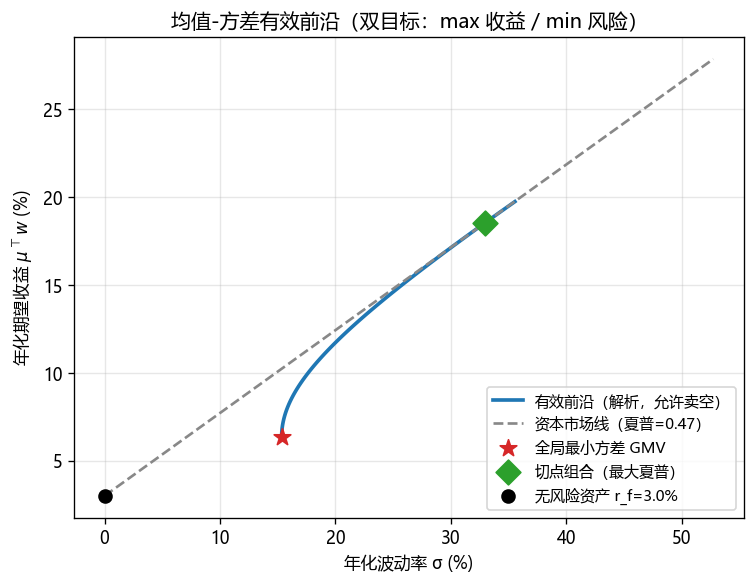
\includegraphics[width=0.74\textwidth]{../figures/efficient_frontier.png}
\caption{均值--方差有效前沿（解析，允许卖空）。红星为 GMV，绿菱为切点组合，
虚线为资本市场线（斜率＝最大夏普比）。}
\label{fig:frontier}
\end{figure}

\begin{figure}[H]
\centering
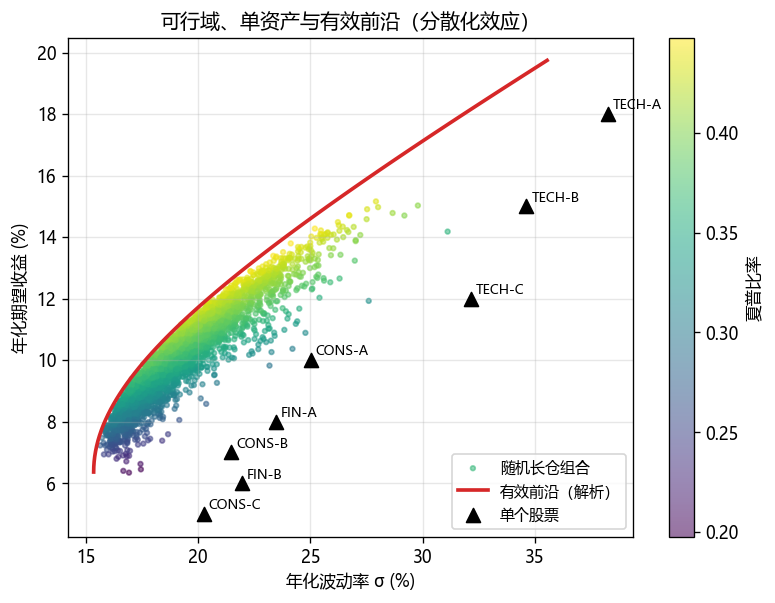
\includegraphics[width=0.78\textwidth]{../figures/frontier_with_assets.png}
\caption{可行域、单资产与前沿。散点为随机长仓组合（按夏普比着色），三角为单只股票。
单资产均位于前沿\emph{内侧}，说明\textbf{分散化}可在同等收益下显著降低风险。}
\label{fig:assets}
\end{figure}

\begin{figure}[H]
\centering
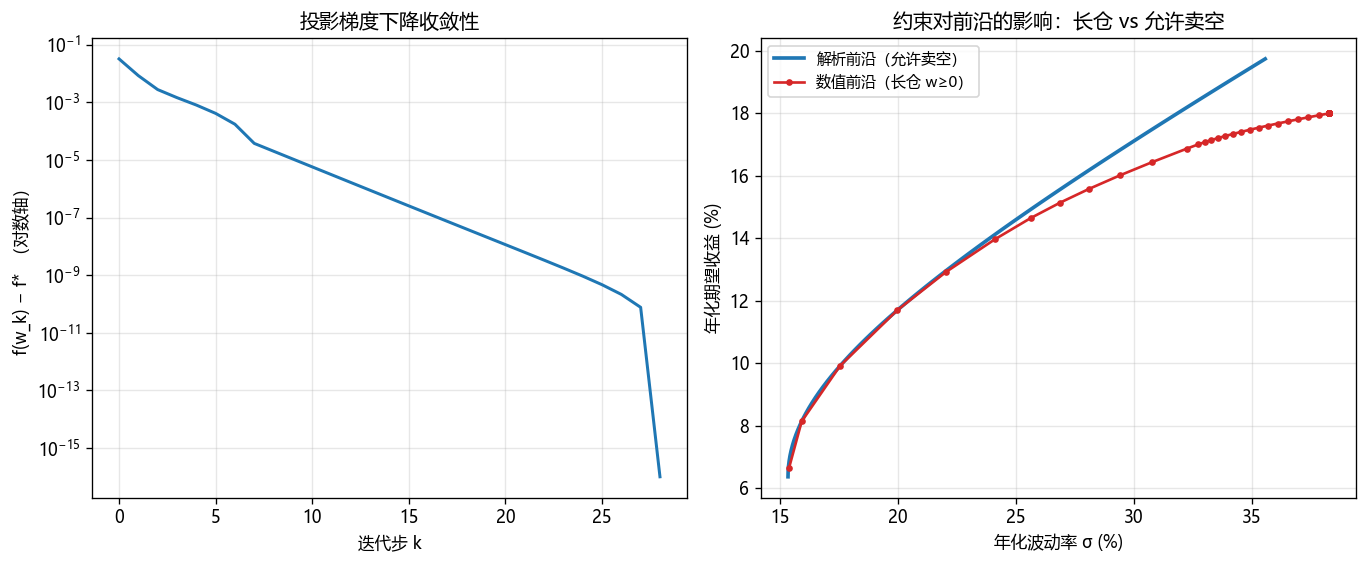
\includegraphics[width=0.92\textwidth]{../figures/pgd_convergence.png}
\caption{左：投影梯度下降的目标值误差 $f(\w_k)-f^\star$（对数轴，呈线性收敛）。
右：长仓（$\w\ge\bm0$）数值前沿位于允许卖空的解析前沿\emph{内侧}，高收益端差距明显，
说明不可卖空约束牺牲了一部分可达收益。}
\label{fig:pgd}
\end{figure}

\begin{figure}[H]
\centering
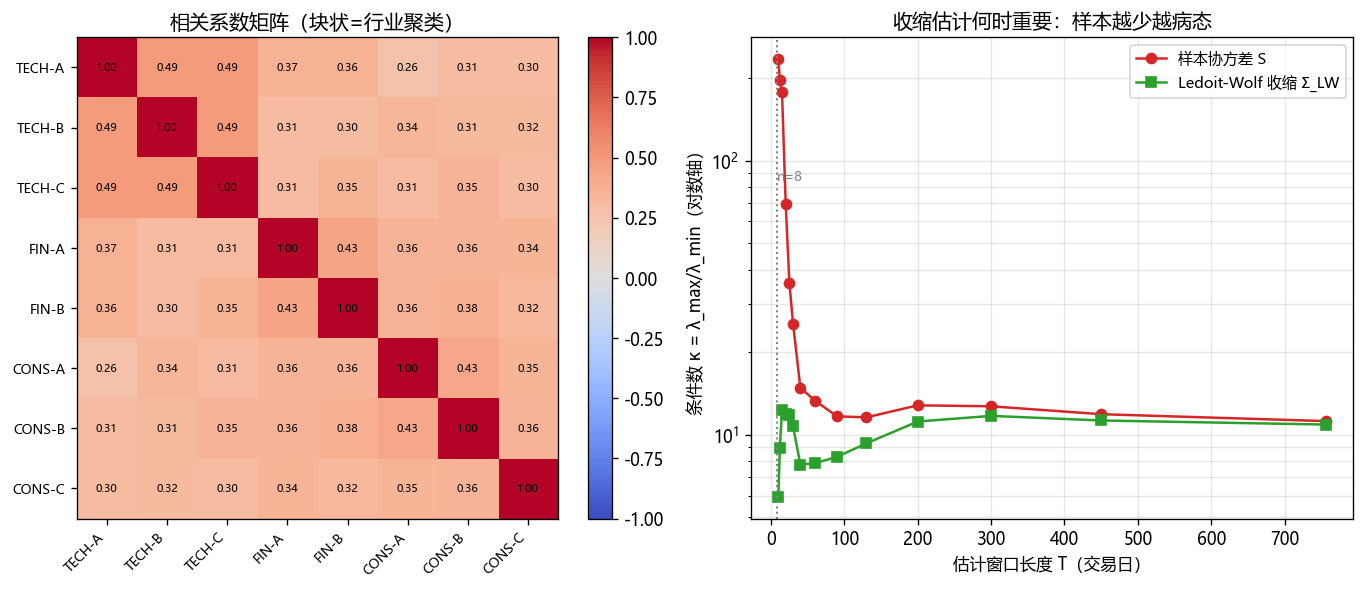
\includegraphics[width=0.92\textwidth]{../figures/covariance_heatmap.png}
\caption{左：相关系数矩阵，行业内相关明显高于行业间（块状结构）。
右：条件数随估计窗口长度 $T$ 的变化——样本越少，样本协方差越病态，
而 Ledoit--Wolf 收缩始终保持良态。}
\label{fig:cov}
\end{figure}

\begin{figure}[H]
\centering
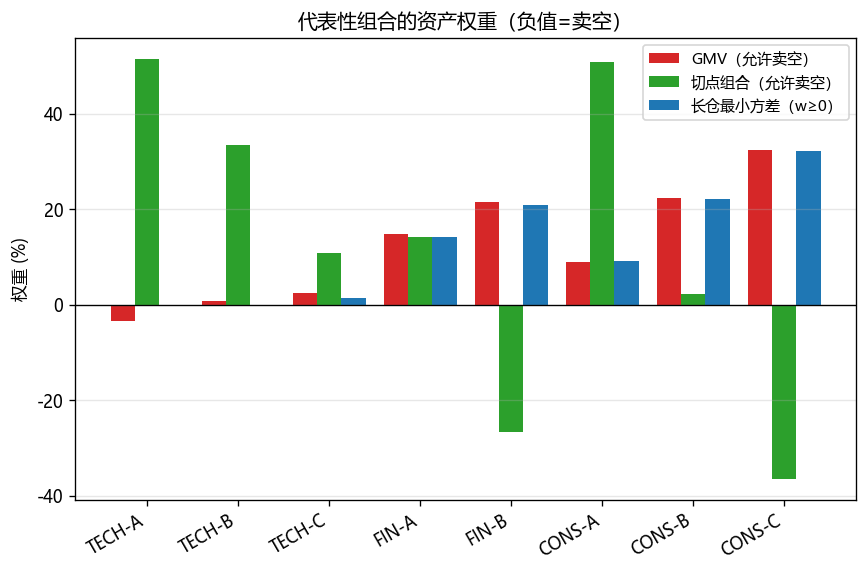
\includegraphics[width=0.80\textwidth]{../figures/weights_allocation.png}
\caption{三种代表性组合的资产权重。切点组合（允许卖空）出现明显负权重（做空低收益资产），
而长仓最小方差组合全部非负——直观展示约束 $\w\ge\bm0$ 的影响。}
\label{fig:weights}
\end{figure}

\paragraph{结果解读。}
GMV 把资金集中到低波动的金融/消费股，年化波动最低；切点组合通过做空低收益资产、
做多高夏普资产取得最高夏普比；加入不可卖空约束后，前沿整体内移、可达收益上限下降。
所有解析结论均通过数值自检（$\sigma^2_{\mathrm{gmv}}=1/C$、权重和为 $1$、KKT 残差 $\approx0$、
自研 PGD 与 \texttt{scipy} 的 SLSQP 解最大偏差 $<10^{-3}$），见 \texttt{results/summary.json}。

% =========================================================================
\section{随机矩阵理论与自助法推断（样本外实验补充）}

\subsection{Marchenko--Pastur 定理与特征值裁剪}

设 $T\times n$ 数据矩阵的行向量为 i.i.d.\ 纯噪声（方差 $\sigma^2$）。当 $T,n\to\infty$、
$q=n/T$ 固定时，样本相关矩阵的特征值依分布收敛到 Marchenko--Pastur 律
\begin{equation}
\rho(\lambda)=\frac{\sqrt{(\lambda_+-\lambda)(\lambda-\lambda_-)}}{2\pi q\,\sigma^2\lambda},
\qquad \lambda_\pm=\sigma^2\bigl(1\pm\sqrt{q}\bigr)^2,
\end{equation}
支撑为 $[\lambda_-,\lambda_+]$。于是凡落入噪声带的样本特征值与纯噪声在统计上不可区分，
只有 $\lambda>\lambda_+$ 的特征值才携带真实相关结构（市场/行业因子）。

\paragraph{裁剪估计量（Bouchaud--Potters 配方）。}
对样本相关阵作特征分解 $C=V\Lambda V\T$，把 $\lambda_i\le\lambda_+$ 的噪声特征值替换为
它们的均值（\textbf{保迹}：$\sum_i\lambda_i'=\tr C=n$），重构 $C'=V\Lambda'V\T$ 后重新归一
使对角恰为 $1$，再乘回样本标准差得 $\Sig_{\mathrm{RMT}}$。

\paragraph{因子估计量。}
只保留 $k=\#\{\lambda_i>\lambda_+\}$ 个信号特征对：
\begin{equation}
C_f=\sum_{i\le k}\lambda_i v_i^{\vphantom{\T}}v_i\T + D,\qquad
D_{jj}=1-\sum_{i\le k}\lambda_i v_{ij}^2=\sum_{i>k}\lambda_i v_{ij}^2\;\ge\;0 ,
\end{equation}
对角残差使 $C_f$ 半正定且对角为 $1$。由迹约束知平均特征值为 $1<\lambda_+$，故必有 $k<n$
（全部特征值超界将使迹超过 $n\lambda_+>n$，矛盾）。

\paragraph{低维警示。}
本项目 $q=8/252\approx0.032$，$\lambda_+\approx1.39$，噪声带很窄。实验中全部 $108$ 个
滚动窗口都只有市场因子（$\lambda\approx3\sim4$）超出 $\lambda_+$，三个行业因子在统计上
与噪声不可分而被一并裁掉——裁剪后的 $\Sig$ 低估行业内相关，反而令切点组合的杠杆更极端
（样本外夏普 $-0.56$，劣于直接用样本协方差）。RMT 是 $n/T$ 较大时的高维武器；低维时
样本协方差本不病态，谱手术的收益预期有限，甚至为负。

\subsection{Circular block bootstrap 与夏普差检验}

单条样本外收益路径给出的夏普比率只是点估计。设 $m$ 个策略的样本外日收益矩阵为
$R\in\R^{T\times m}$，第 $b$ 次重采样以块长 $\ell$（取再平衡周期 $21$ 天）生成环形块索引：
块起点独立同分布于 $U\{0,\dots,T-1\}$，每块取连续 $\ell$ 天（模 $T$ 回绕），拼接后截断到
长度 $T$——块内的波动聚集等时序依赖得以保留。

关键设计是\textbf{联合重采}：同一组索引同时作用于 $R$ 的全部 $m$ 列，保留策略间的截面
相关。如此夏普差 $\Delta_b=\widehat{\mathrm{SR}}^{(i)}_b-\widehat{\mathrm{SR}}^{(j)}_b$
中共同的市场波动相互抵消，检验才有功效；若各列独立重采，$\Delta$ 的方差将被严重高估。
每个 resample 内\textbf{整段重算}年化夏普（均值与波动在同一 resample 内相关，不可分别
抽样再组合）。双侧 $p$ 值采用 $(\#+1)/(B+1)$ 修正以避免报出 $p=0$。

\paragraph{实验结论。}
$B=2000$ 次重采样下，全部策略相对等权 $1/N$ 的 $\Delta\mathrm{Sharpe}$ 置信区间均横跨
$0$（最小 $p=0.079$）：在一条 $9$ 年的样本外路径上，连使用真实 $\muv$ 的 Oracle 切点
组合都无法在统计上显著胜过 $1/N$（$p=0.85$）。这把 DeMiguel et al.\ (2009) 的结论又推进
一步——不仅估计误差会摧毁样本内最优，而且单条路径的噪声之大，使任何“跑赢”都难以被证实。

% =========================================================================
\section{给期望收益开药方、维数相变与最优协方差}

\subsection{Jorion 的 Bayes--Stein 收缩}

既然实验证明 $\muv$ 的估计误差是样本外失败的元凶，经典药方是对 $\muv$ 本身做收缩
（与 Ledoit--Wolf 对 $\Sig$ 的收缩完全对仗）。Jorion (1986) 把样本均值 $\hat\muv$
向 GMV 隐含收益 $\mu_0=\frac{\one\T\Sinv\hat\muv}{\one\T\Sinv\one}$ 收缩：
\begin{equation}
\muv_{\mathrm{BS}}=(1-\hat w)\,\hat\muv+\hat w\,\mu_0\one,\qquad
\hat w=\frac{n+2}{(n+2)+T\,(\hat\muv-\mu_0\one)\T\Sinv(\hat\muv-\mu_0\one)}\in(0,1].
\end{equation}
收缩强度由 $\hat\muv$ 偏离目标的马氏距离决定：偏离越像噪声（相对于 $T$ 个样本的
抽样误差），收缩越狠。实验中 $\hat w\in[0.39,0.81]$，$\muv$ 的平均估计误差从
$0.77$ 降到 $0.49$（年化 $\ell_2$ 范数），切点组合换手率近乎减半。

\subsection{Black--Litterman 均衡先验与"无观点定理"}

从"市场组合即等权 $\w_{\mathrm{eq}}=\one/n$"反向优化出均衡隐含收益
\begin{equation}
\bm\pi=r_f\one+\delta\,\Sig\,\w_{\mathrm{eq}},\qquad
\delta=\frac{\bar r_{\mathrm{mkt}}-r_f}{\sigma^2_{\mathrm{mkt}}}.
\end{equation}
以 $\bm\pi$ 为输入的切点组合权重为 $\w\propto\Sinv(\bm\pi-r_f\one)=\delta\,\w_{\mathrm{eq}}$，
归一化后\textbf{恰好还原} $\w_{\mathrm{eq}}$（$\delta$ 在归一化中消去）——不持有观点的
贝叶斯投资者就该持有市场。实验对全部 $108$ 个滚动窗口数值验证：
$\max|\w_{\mathrm{BL}}-\one/n|\approx10^{-15}$（机器精度）。

进一步做收缩路径扫描 $\muv_\varphi=(1-\varphi)\bm\pi+\varphi\hat\muv$：最优在
$\varphi^*=0$（纯均衡），且中间 $\varphi$ 并非平滑过渡而是剧烈震荡——当混合后的
超额收益向量 $\muv_\varphi-r_f\one$ 接近零向量时，切点归一化因子 $\one\T\Sinv(\muv_\varphi-r_f\one)$
趋零，权重爆炸。在这条样本路径上，样本信息掺入多少都只会伤害组合。

\subsection{维数相变：RMT 的翻案}

固定 $T=252$、把资产数从 $n=8$ 扫到 $200$（$q=n/T$ 从 $0.03$ 到 $0.79$），数据
生成过程同构、真实信号秩恒为 $4$。以 GMV 的样本外实现波动衡量 $\hat\Sig$ 的质量
（不经过 $\muv$）：$q$ 小时四种估计并列；$q\to1$ 时样本协方差条件数爆炸
（中位数 $\approx1.1\times10^4$），其 GMV 波动回升到与等权持平——\textbf{维数带来的
分散化红利被估计误差悉数吃掉}；而 MP 裁剪与 PCA 因子估计只保留 $O(1)$ 个信号特征对，
对维数免疫，波动持续下降（$18\%\to9\%$）。RMT 在 $q$ 小时是误伤真实因子的手术刀，
在 $q$ 大时是唯一的救命稻草——任何估计量都有其适用边界。

\subsection{最优协方差：解析非线性收缩}

线性收缩（LW2004）把特征值朝同一常数拉、RMT 裁剪把噪声压成台阶，都是"一刀切"。
Ledoit--Wolf (2020) 的\textbf{非线性收缩}保持特征向量不变，只对每个样本特征值 $\lambda_i$
施加一个最优的、连续变化的缩放
\begin{equation}
\tilde d_i=\frac{\lambda_i}{\bigl(\pi c\lambda_i\tilde f(\lambda_i)\bigr)^2
+\bigl(1-c-\pi c\lambda_i\,\mathcal H\tilde f(\lambda_i)\bigr)^2},\qquad c=\tfrac{p}{n},
\end{equation}
其中样本谱密度 $\tilde f$ 及其 Hilbert 变换 $\mathcal H\tilde f$ 由带宽 $h=n^{-1/3}$ 的
Epanechnikov 核估计。该式是 Frobenius 范数下最优旋转等变估计的渐近实现：小特征值
（被噪声压低）被抬高、大特征值（被高估）被压低。实验用纯 numpy 从零实现（特征分解
$+$ 核密度 $+$ Hilbert 变换解析式 $+$ 上式），并数值验证其与样本协方差对易（仅改特征值，
相对残差 $\sim10^{-15}$）。效果上 NLS"从不更差"：$n=8$ 时贴近样本协方差，$n=200$ 时将
条件数中位数从 $10994$ 压到 $217$、GMV 实现波动从 $17.5\%$ 降到 $9.4\%$，紧贴因子模型的
最优表现，却无需假设因子数、也不在低维误伤真实信号——为协方差估计给出理论与实践统一的最优解。

% =========================================================================
\section{结论}

本项目以矩阵算法为主线，完整走通了一个量化金融多目标规划问题：从双目标建模、标量化，
到拉格朗日/KKT 闭式解（依托 Cholesky 与特征分解）、再到不可卖空约束下从零实现的投影梯度
下降（含单纯形投影推导与收敛性分析），最后用 Ledoit--Wolf 收缩把机器学习的正则化思想
引入协方差估计。在此基础上，样本外滚动回测量化了 $\muv$ 估计误差的真实代价，随机矩阵
理论与 block bootstrap 揭示了协方差谱手术的低维局限与回测结论本身的统计不确定性，
Bayes--Stein 收缩与 Black--Litterman 均衡先验给出了 $\muv$ 的可行药方，维数扫描画出了
每种估计量的适用边界，解析非线性收缩则为协方差估计给出理论最优解。理论推导、代码实现、
图像与数值自检相互印证，可作为矩阵算法课程的完整范例。

\end{document}
